\begin{frame}[t]{Genie-2}
  \centering\vspace{0.06em}
  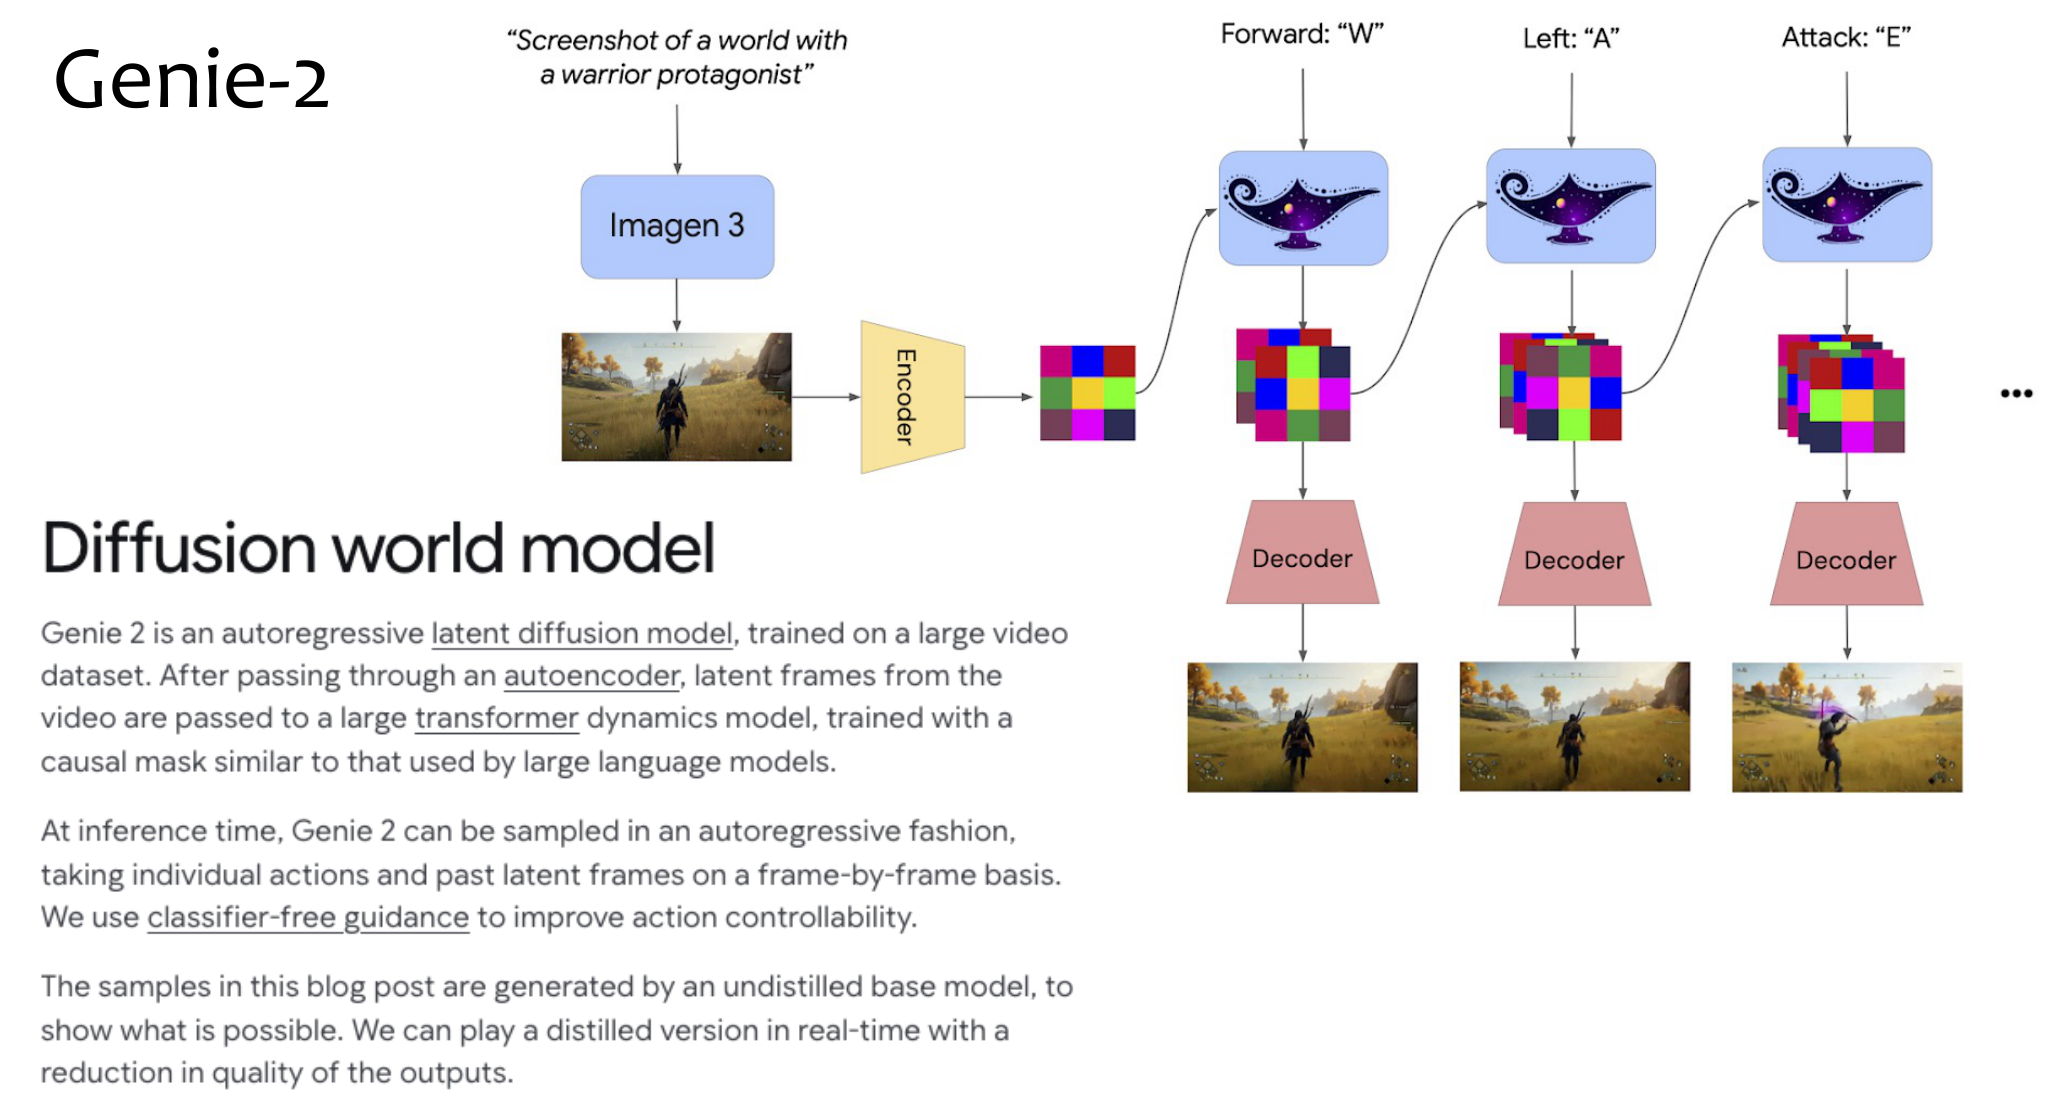
\includegraphics[width=\linewidth,height=0.86\textheight,keepaspectratio]{assets/New-Lecture-Video_Generation/cmu10423_lecture26_world_models_slide29.png}\\[0.28em]
  {\scriptsize Source: CMU Lecture 26, World Models.}
\end{frame}

\begin{frame}[t]{Genie-2}
  \begin{itemize}
    \item The technical description of Genie-2 is rather vague.
    \item This could indicate that the primary change is \textbf{scale}:
    \begin{itemize}
      \item \textbf{more parameters}
      \item \textbf{more training data}
    \end{itemize}
  \end{itemize}
  \vfill
  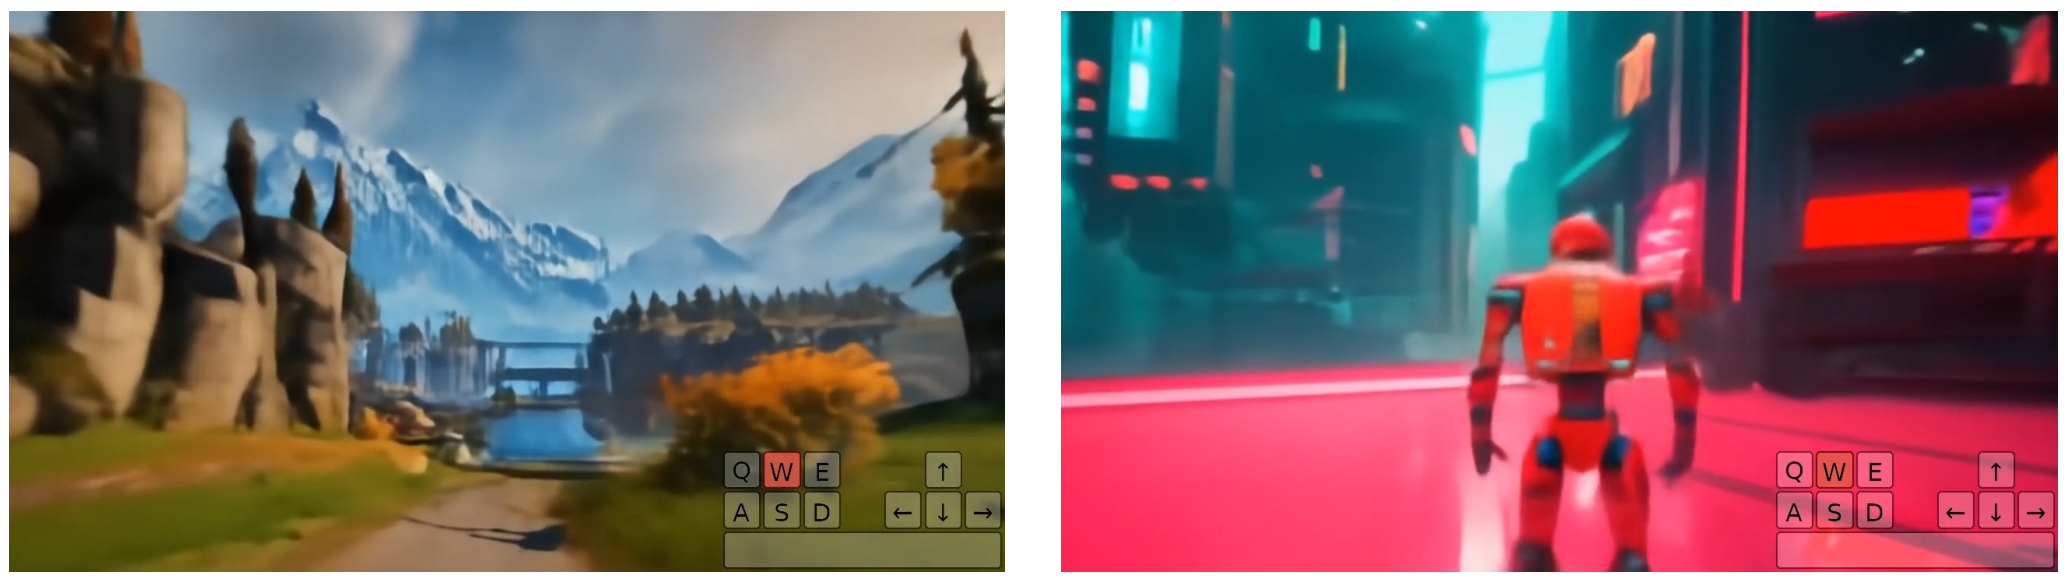
\includegraphics[width=0.85\linewidth,height=0.85\textheight,keepaspectratio]{assets/New-Lecture-Video_Generation/cmu10423_lecture26_world_models_slide30.png}\\[0.28em]
  {\scriptsize Source: CMU Lecture 26, World Models.}
\end{frame}

\begin{frame}[t]{Genie-3}
\centering
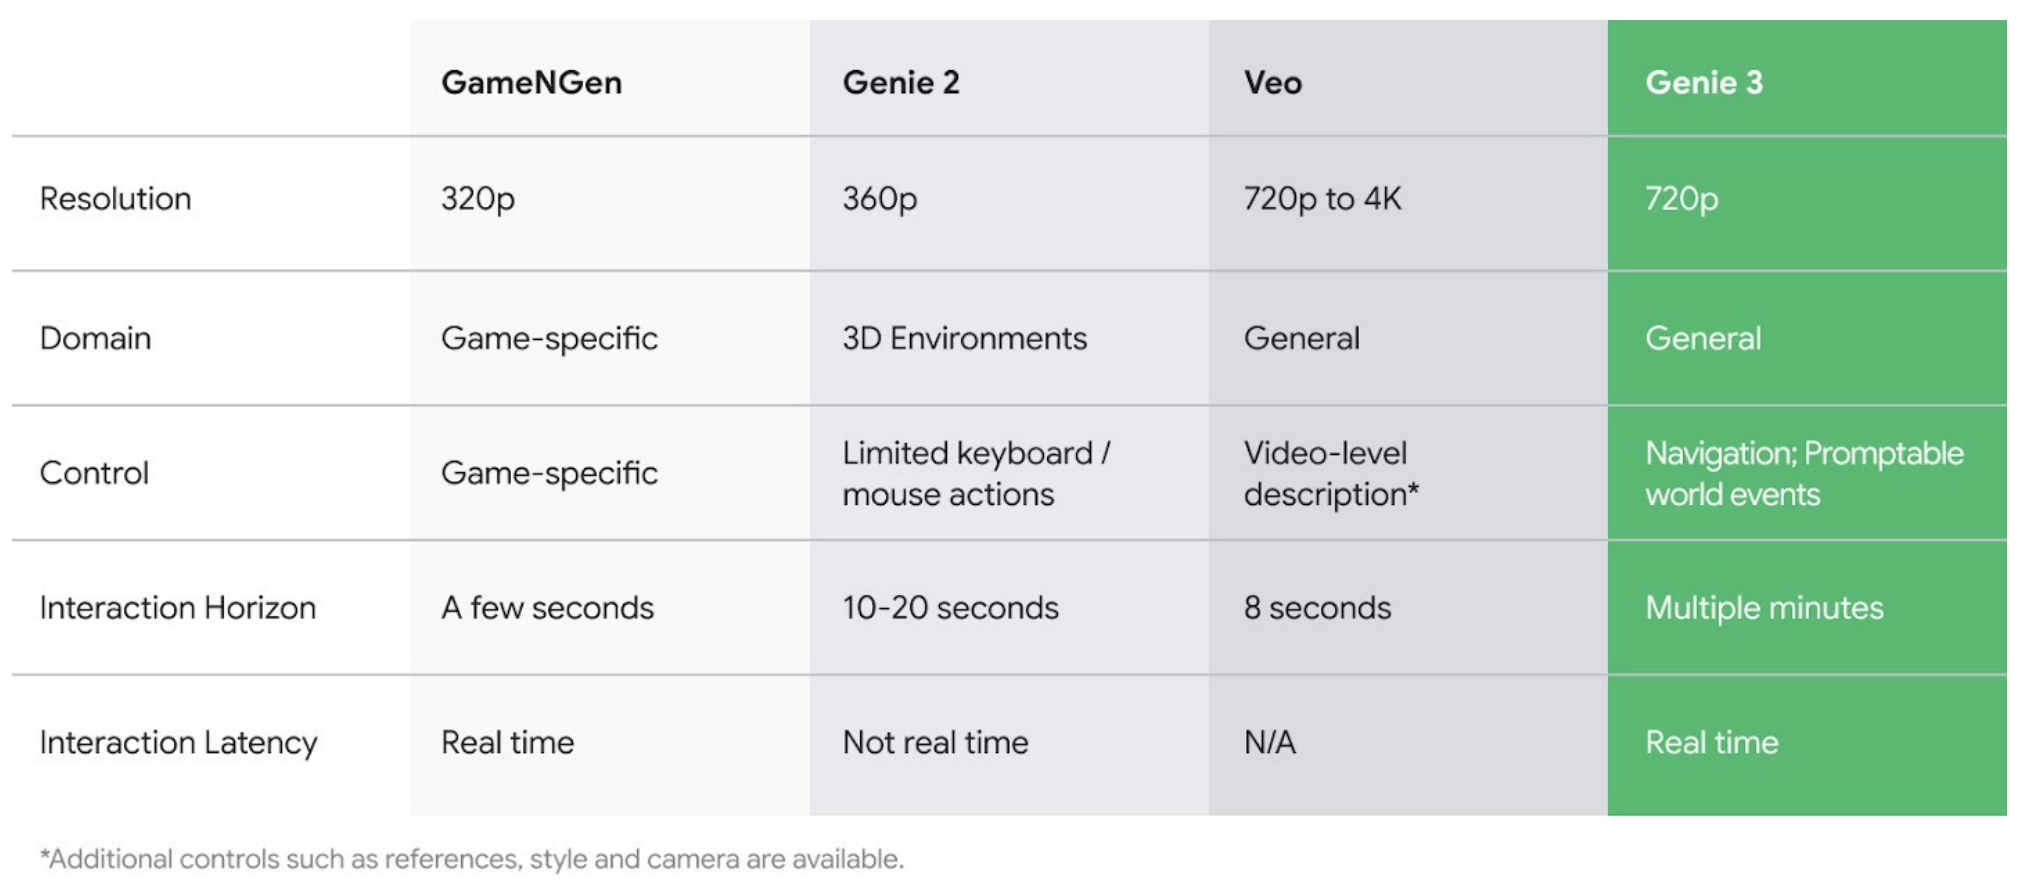
\includegraphics[width=0.85\linewidth,height=0.95\textheight,keepaspectratio]{assets/New-Lecture-Video_Generation/cmu10423_lecture26_world_models_slide31.png}\\[0.28em]
{\scriptsize Source: CMU Lecture 26, World Models.}
\end{frame}

\begin{frame}[t]{Genie-3}
  \centering
  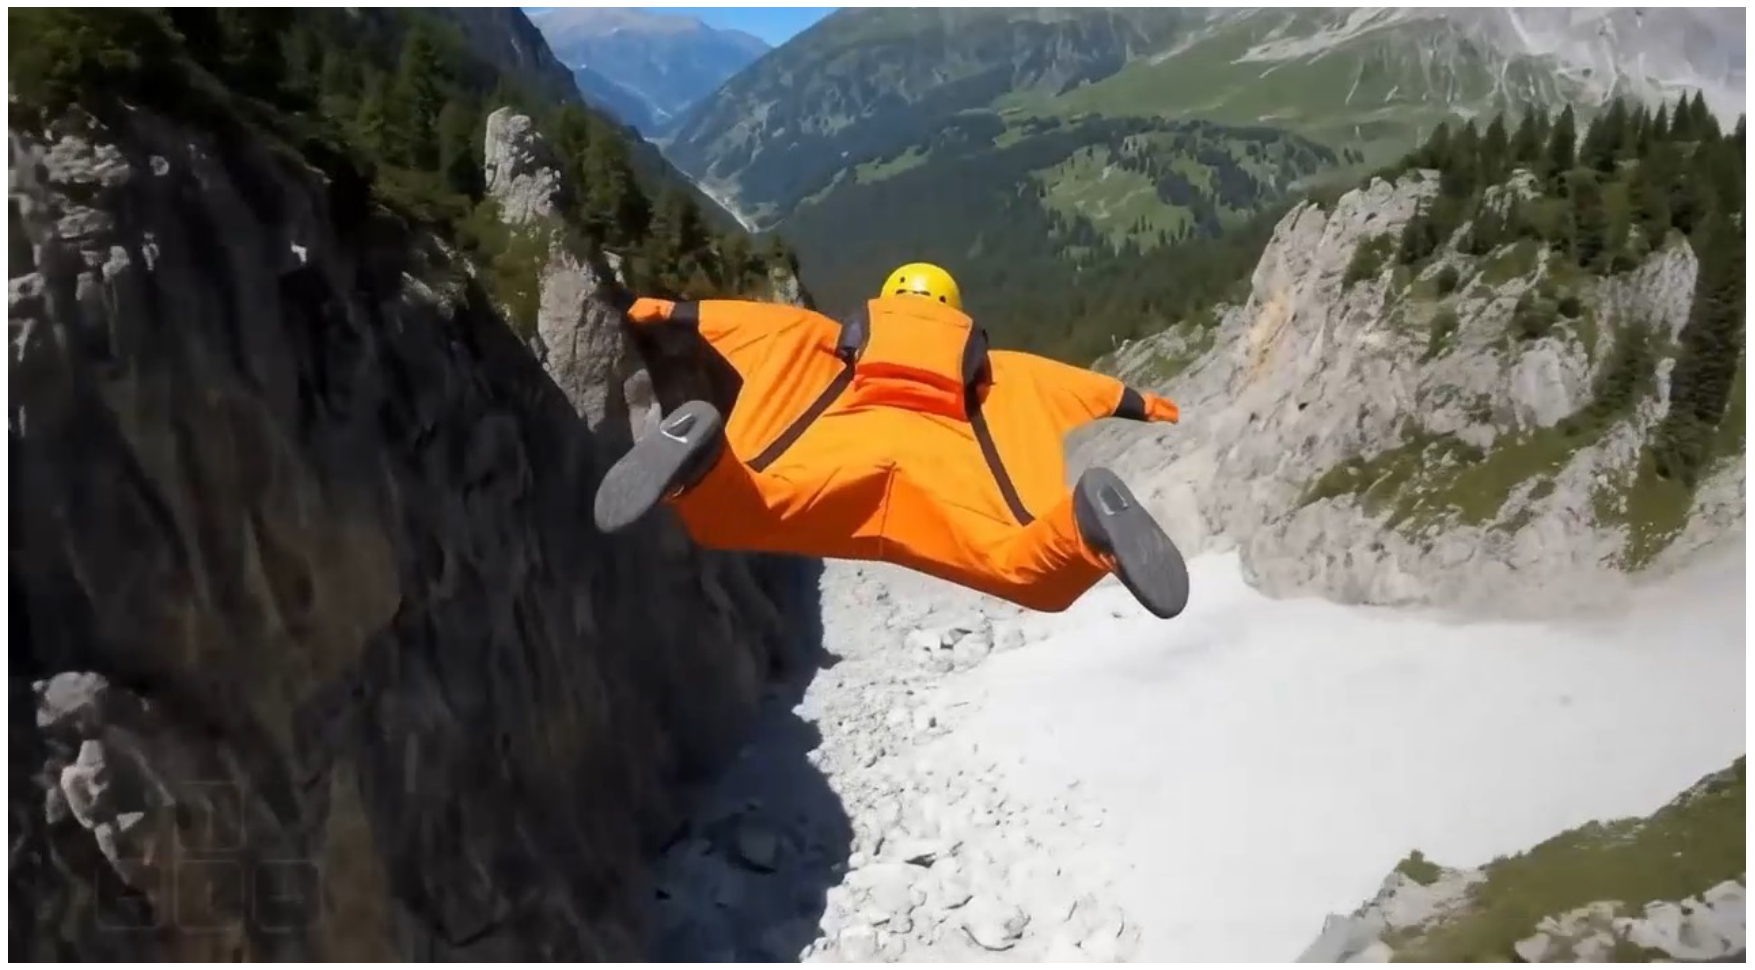
\includegraphics[width=0.85\linewidth,height=0.85\textheight,keepaspectratio]{assets/New-Lecture-Video_Generation/cmu10423_lecture26_world_models_slide32.png}\\[0.28em]
  {\scriptsize Source: CMU Lecture 26, World Models.}
\end{frame}

\begin{frame}[t]{Genie-3: Limitations}
  \begin{itemize}\itemsep0.37em
    \item Interaction window is limited to a short duration (a few minutes).
    \item Actions are (likely) latent and from a fixed set; defining new actions is not possible.
    \item Prompting for changes in the world is possible and represents an open set; this creates an asymmetry between the closed action set and the open world change set.
    \item Limited to one character (at least that seems to be the case).
    \item Fundamentally just a video model: no game-engine-interpretable world representation (e.g., point cloud, mesh, Gaussian splatting) is provided.
    \item Extremely high computational demands.
  \end{itemize}
\end{frame}
